\subsubsection{Erster Test des Gehäuses}\label{hw_case_ersterTest}
Zur Erstellung des Gehäuses haben wir die Maße des Bildschirms als Anhaltspunkt genommen. Das Gehäuse befand sich zu diesem Zeitpunkt bei Felix Kuschel, der die Messungen vornahm. Der Bildschirm hatte an der Hinterseite eine Erhebung, weshalb er diese ebenfalls ausgemessen hatte. Die Maße beliefen sich dann auf:
\begin{itemize}
	\item 255,5 mm Breite
	\item 167 mm Höhe
	\item Kantenradius 10 mm
\end{itemize}
	\begin{figure}[h!t]
		\includegraphics[width=1\textwidth]{img/abmessungen_gehäuse.jpg}
		\caption[Abmessungen Bildschirm Rückseite]{Abmessungen Bildschirm Rückseite}
		\label{fig:screen-back-01}
	\end{figure}
	Die Maße an der Rückseite übermittelte er Manuel Starz als Bild. Anhand dieser Maße hat Manuel Starz dann in Fusion 360 eine Grundplanzeichnung erstellt und ein 3D-Modell gefertigt.\par	
	Nach Überprüfung der Maße mussten wir dann allerdings feststellen, dass der zur Verfügung stehende 3D-Drucker, ein Ender 3 Pro der Firma Creality3D, ein maximales Druckvolumen von 235x235x220mm besitzt und somit das Gehäuse nicht wie ursrpünglich geplant aus einem Stück sondern in mehreren Teilen gedruckt werden musste. Hierfür war eine Änderung der Konstruktion von Nöten. Das Gehäuse besteht nun aus vier Teilen, zwei bilden jeweils die Seitenwände während zwei den Deckel des Gehäuses bilden. Die Teile werden mit langen M3 Senkkopfschrauben verbunden, die zusätzlich als Verschluss des Gehäuses dient. \par
	
	\begin{figure}[h!]
		\includegraphics[width=1\textwidth]{img/druck_gehäuse_001.png}
		\caption[Platzierung der beiden Gehäusewände in CURA]{Platzierung der beiden Gehäusewände in CURA}
		\label{fig:print-case-test_01}
	\end{figure}
	\begin{figure}[h!]
		\includegraphics[width=1\textwidth]{img/druck_gehäuse_002.png}
		\caption[Verschiebung der Modelle entlang der Z-Achse um 45mm]{Verschiebung der Modelle entlang der Z-Achse um 45mm}
		\label{fig:print-case-test_02}
	\end{figure}
	\begin{figure}[h!]
		\includegraphics[width=1\textwidth]{img/druck_gehäuse_002.png}
		\caption[Slicen der Modelle]{Slicen der Modelle}
		\label{fig:print-case-test_03}
	\end{figure}
	\begin{figure}[h!]
		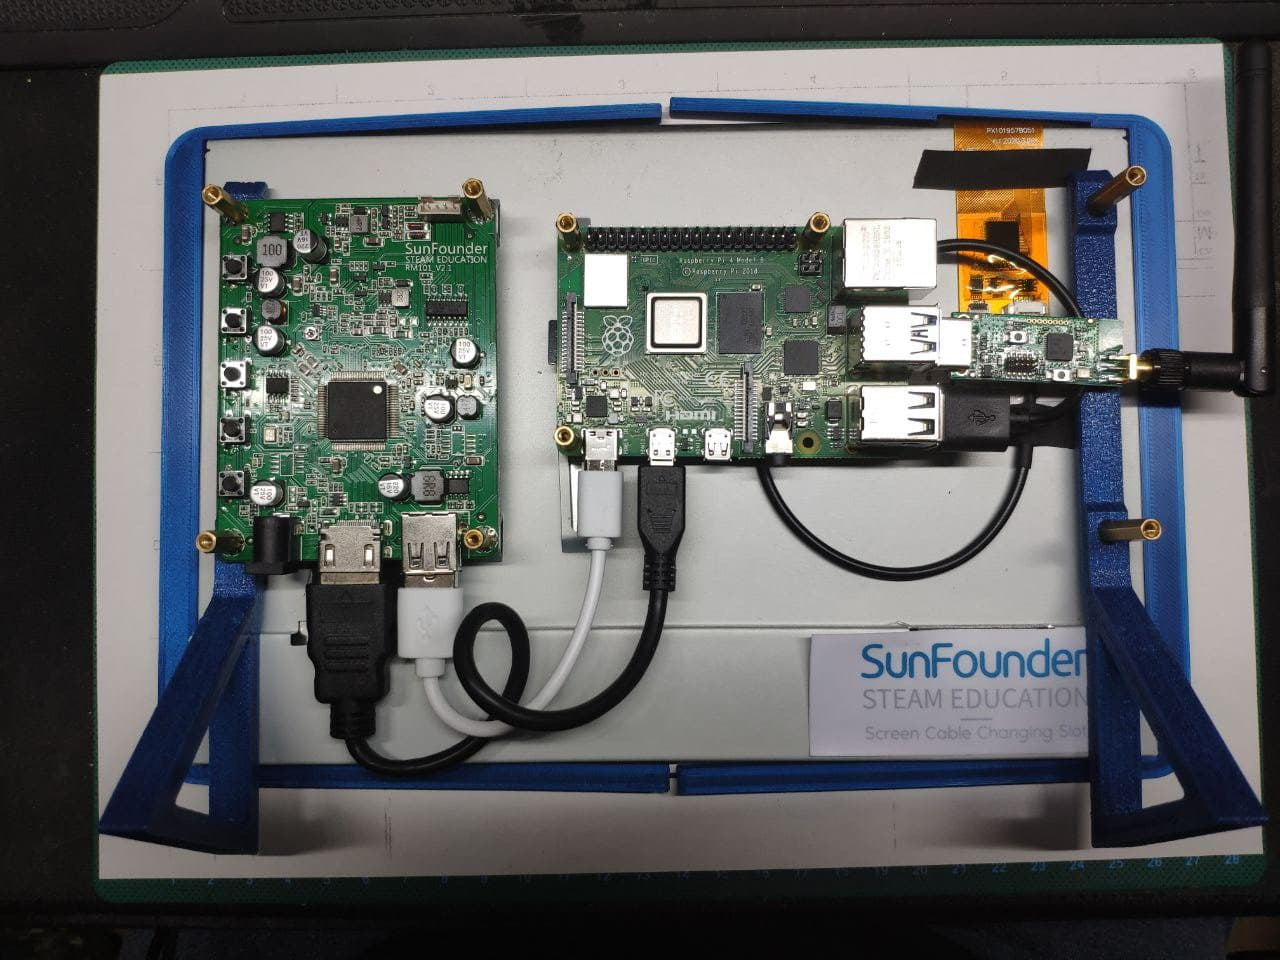
\includegraphics[width=1\textwidth]{img/testdruck_an_bildschirm.jpg}
		\caption[Passung des Testdrucks]{Passung des Testdrucks}
		\label{fig:print-case-test_04}
	\end{figure}
	Um die Genauigkeit der Konstruktion zu testen, hat Manuel Starz eine 5 Millimeter hohe Testschablone ausgedruckt, die an den Bildschirm angelegt werden kann. Diese entstand mit Hilfe des Slicers CURA (vgl. Abbildung \ref{fig:print-case-test_01}), in dem die Modelle der beiden Seitenteile so angeordnet wurden, dass lediglich 5 Millimeter des Teils im druckbaren Bereich des Druckers verblieben (vgl. Abbildung \ref{fig:print-case-test_02}).\par